 \documentclass{report}
 
\usepackage[utf8]{inputenc} 
\usepackage[T1]{fontenc}      
\usepackage[top=2.0cm, bottom=3cm, left=3.0cm, right=3.0cm]{geometry}
\usepackage{graphicx}
\usepackage{wrapfig}
\usepackage{amsmath,esint }
\usepackage{amssymb}
\graphicspath{{figures/}{../figures}}

\newcommand*\dif{\mathop{}\!\mathrm{d}}
\newcommand*\diver{\mathop{}\!\mathrm{div}}
\newcommand*\grad{\mathop{}\!\mathrm{grad}}

\begin{document}

\section*{Sillage d'un avion}

\begin{itemize}

	\item[$\circ$] On retrouve l'équation d'Alembert à partir de trois équation. Sur la masse volumique et la compressibilité :
	\begin{align*}
		\mu = \chi_sp\rho_0
	\end{align*}
	Sur l'équation de la conservation de la masse :
	\begin{align*}
		\frac{\partial \mu}{\partial t}+\grad(p)=0
	\end{align*}
	et l'équation d'Euler :
	\begin{equation}
		\rho_0\frac{\partial \vec{v}}{\partial t}+\vec{\grad}(\vec{v})=0
	\end{equation}
	On trouve alors une équation d'Alembert sur $\mu$, $\vec{v}$ et $p$, avec une célérité $c=1/\sqrt{\chi_s\rho_0}$

	\item[$\star$] Il faut raisonner en calculant l'écart entre 2 "bips" émis par l'avion à la période $T$. Soit $t_1=t$ et $t_2=t+T$ les temps où l'avion émet 2 bips à partir du temps $t$. Soient $t'_1$ et $t'_2$ les temps auxquels sont reçus les signaux par l'observateur. Comme l'onde se propage à la vitesse $c$ : $t'_1=t_1+d_1/c$ et $t'_2=t_2+d_2/c$ avec $d_1$ et $d_2$ les distances entre l'avion et l'observateur. La période entendue par l'observateur est :
	\begin{align*}
		T'=t'_2-t'_1=\frac{h}{c}\left(\frac{1}{\sin\theta(t_2)}-\frac{1}{\sin\theta(t_1)} \right) +T=-\frac{h\delta\theta\cos\theta(t_1)}{\sin^2\theta(t_1)} +T 
	\end{align*}
	En notant $\delta\theta=\theta(t_2)-\theta(t_1)\ll1$. Pour trouver $\delta\theta$ :
	\begin{align*}
		\tan\theta(t_2)-\tan\theta(t_2)=h\left(\frac{1}{x(t_1)}-\frac{1}{x(t_1)-vT} \right) =-\frac{vTh}{x(t_1)}=\frac{\delta\theta}{\cos^2\theta(t_1)}
	\end{align*}
	Donc $\delta\theta=-vT\sin^2\theta(t_1)/h$
	On trouve alors au final :
	\begin{align*}
		T'=T\left(1-\frac{v}{c}\cos\theta \right) 
	\end{align*}
	\item[$\star$] Les ondes émises sont sous forme de sphère, donc en théorie tout l'espace peut être atteint par le bruit de l'avion s'il vole depuis un temps infini. On entend l'avion avant qu'il passe devant l'observateur.

	\item[$\diamond$] L'onde émise à l'instant $t$ parcourt une distance $d(t)=\sqrt{x^2+h^2}$ avant d'arriver à l'observateur. Donc :
	\begin{align*}
		t'=t+\sqrt{\frac{h^2}{c^2}+\frac{v^2t^2}{c^2}}
	\end{align*}

\begin{figure}[h!]
\centering
		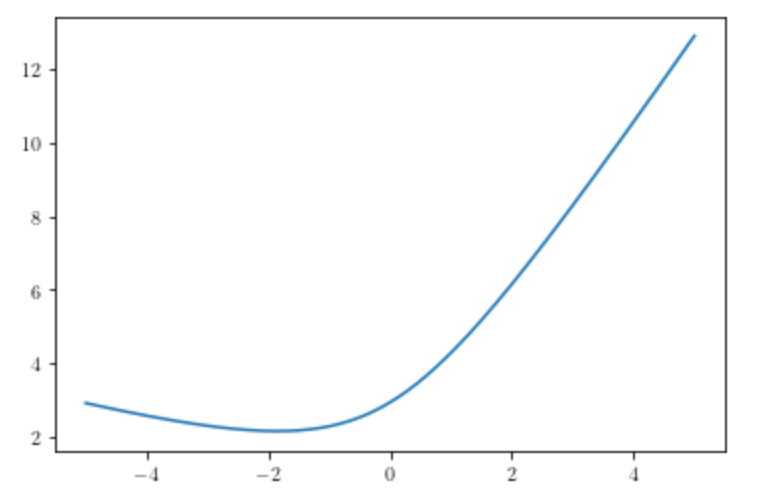
\includegraphics[scale=0.5]{onde_choc.png}
\end{figure}	
	
	\item[$\diamond$] Si $\dif t'/\dif t=0$, à ce moment là le temps d'arrivée des ondes est le même $\forall t$, donc toutes les ondes arrivent en même temps. Il y a un bang !
	
	\item[$\diamond$] $t'_0$ correspond au moment où le bang est perçu par l'observateur, donc d'après la question précédente, correspond au moment où $f'(t_0)=0$.
	\begin{equation}
		f'(t)=1+\frac{v^2t/c^2}{\sqrt{h^2/c^2+v^2t^2/c^2}}
	\end{equation}
	En résolvant l'équation, on trouve que :
	\begin{align*}
		t_0=-\frac{h}{v}\frac{1}{\sqrt{v^2/c^2-1}}
	\end{align*}
	Et :
	\begin{align*}
		t'_0=h\sqrt{1/c^2-1/v^2}
	\end{align*}
	Les positions de l'avion sont $x_0=-h\frac{1}{\sqrt{v^2/c^2-1}}$ et $x'_0=h\sqrt{v^2/c^2-1}$
	
	\item[$\diamond$] L'observateur entend l'avion une fois qu'il se trouve dans le cône dans lequel les ondes sonores sont émises. Il n'entend donc pas l'avion tant qu'il n'a pas entendu le bang. Les sons perçus entre $t'_0$ et $t'_0+\Delta t'$ ont été émis entre $t_0$ et $t_0+\Delta t$. DOnc :
	\begin{align*}
		t'_0+\Delta t'=f(t_0+\Delta t)=f(t_0)+f'(t_0)\Delta t+\frac{1}{2}f''(t_0)\Delta t^2=t'_0+\frac{1}{2}f''(t_0)\Delta t^2
	\end{align*}
	Donc : 
	\begin{align*}
		\Delta t=\sqrt{\frac{2\Delta t'}{f''(t_0)}}, \quad f''(t_0)=\frac{v^2h^2}{c^4(\frac{h^2}{c^2}+\frac{h^2}{v^2-c^2})^{3/2}}
	\end{align*}
	On trouve $\Delta t=0,83$s, cad que le son a bien été compressé (le son perçu est 8 fois plus court). 
	
	\item[$\diamond$] La région atteinte par l'onde sonore émise par l'avion à un instant donné est l'intérieur d'un cône d'angle au sommet $2\theta$ et de sommet le nez de l'avion. 
	
	\item[$\diamond$] L'enveloppe des ondes sonores émises au cours du temps est un cône tangent aux surfaces d'ondes sphériques marquant l'arrivée en un point. On trouve facilement la relation :
	\begin{align*}
		\sin\theta=\frac{c}{v}
	\end{align*}
	Sur la photo, on mesure $\theta\simeq15^\circ$. On a donc $v\simeq352$m.s$^{-1}$. L'avion a juste franchi le mur du son.

\end{itemize}

\section*{Pavillon acoustique}

\begin{itemize}

\item[$\diamondsuit$] Approximation acoustique : $v\ll c$.

\item[$\diamondsuit$] La compressibilité devient $\chi_s=\frac{1}{V}\frac{\partial V}{\partial P}=-\frac{1}{p(x,t)}\frac{\Psi(x+dx,t)S(x+dx)\Psi(x,t)S(x)}{S(x)dx}=-\frac{1}{S(x)p(x,t)}\frac{\partial \Psi(x,t)S(x)}{\partial x}$. On trouve ensuite :
\begin{align*}
	p(x,t) = -\frac{1}{\chi_s}\left(\frac{\partial \Psi}{\partial x}+\Psi(x,t)\frac{\partial }{\partial x}\left[\ln S(x) \right]  \right)
\end{align*}

\item[$\diamondsuit$] L'équation d'Euler :
\begin{align*}
	\frac{\partial^2\Psi}{\partial t^2}+\frac{1}{\rho_0}\frac{\partial p}{\partial x}=0
\end{align*}
On trouve alors :
\begin{align*}
	\frac{\partial^2\Psi}{\partial t^2}-\frac{1}{\chi_s\rho_0}\frac{\partial^2 \Psi}{\partial x^2}=-\frac{\partial}{\partial x}\left(\Psi \frac{\partial \ln S(x)}{\partial x} \right) 
\end{align*}
Même chose pour la pression :
\begin{align*}
	\frac{\partial^2p}{\partial t^2}-\frac{1}{\chi_s\rho_0}\frac{\partial^2 p}{\partial x^2}=-\frac{\partial}{\partial x}\left(p \frac{\partial \ln S(x)}{\partial x} \right) 
\end{align*}

\item[$\diamondsuit$] L'équation de conservation de la masse devient :
\end{itemize}

Le pavillon a une allure exponentielle : $S(x)=S_0\exp(ax)$. On suppose que l'onde est une onde plane, progressive et monochromatique : $p(x,t)=p_0\exp\left(j[\omega t-kx] \right)$. On notera la vitesse de déplacement $v(x,t)=\partial\Psi/\partial t$.

\begin{itemize}

\item[$\diamondsuit$]  Quelle est alors l'équation de dispersion ? Montrer qu'il ne peut pas y avoir de propagation en dessous d'une certaine pulsation de coupure $\omega_c$.

\item[$\diamondsuit$] Donner les expression de $v(x,t)$, $p(x,t)$, puis celle de l'énergie acoustique $\varepsilon(x,t)$ et du vecteur de Poyting $\Pi(x,t)$.

\end{itemize}

\newpage

\section*{Impédance acoustique}

On considère une onde acoustique se propageant selon les $x$ croissants dans un milieu 1 et atteignant le milieu 2 en $x=0$. Les milieux 1 et 2 sont caractérisés respectivement par une masse volumique $\rho_1$ et $\rho_2$ et une célérité des ondes acoustiques $c_1$ et $c_2$. 

\subsubsection*{Échographie}

\begin{itemize}
	
	\item[$\spadesuit$] Rappeler l'équation d'Alembert vérifiée par la surpression $p(x,t)$ et la vitesse $v(x,t)$ dans un milieu homogène. Quelles sont les solutions générales ? Qu'appelle t-on les ondes planes progressives monochromatiques ?	
	
	\item[$\spadesuit$] Écrire les relations que vérifient la vitesse et la surpression à l'interface en $x=0$. Que se passe t-il lorsque l'onde arrive de par la gauche sur l'interface $1\longrightarrow2$ pour que ces relations soient vérifiées ? Justifier de l'existence d'une onde réfléchie et transmise.
	
	\item[$\spadesuit$] En déduire les coefficients de réflexion $r$ et de transmission $t$.
	
	\item[$\spadesuit$] Pourquoi dont-on mettre un gel sur entre la sonde et le corps durant une échographie ? 
		
\end{itemize}

\subsubsection*{Isolation phonique}

On suppose qu'il y a désormais une paroi de masse surfacique $\mu$ à l'interface entre les deux milieux, qui sont supposées être identiques ($\rho_1=\rho_2$ et $c_1=c_2$). Cette paroi se meut librement et sans frottement. 

\begin{itemize}
	
	\item[$\clubsuit$] Que deviennent les relations de passage précédentes ? En déduire les coefficients de réflexion et de transmission dans ce cas-là. 
	
	\item[$\clubsuit$] Calculer $T=\mid t\mid^2$ et tracer l'allure de la courbe $G_{db}=20\log\left[T(\omega) \right]$ en fonction de $\log(\omega)$. Quelle est la fréquence de coupure ?
	
	\item[$\clubsuit$] De combien doit être l'épaisseur d'un mur de béton entre deux logements d'un appartement pour que l'atténuation soit atténuée de 50dB à 300Hz ? On donne $\rho_{béton}=2300$kg.m$^{-3}$. 
	
\end{itemize}


\end{document}
